% date: 2024-09-21
% Author: Bai Junhao
% Email: bjh2001@connect.hku.hk
% The University of Hong Kong

\section{Peter buttered the burnt toast}

\subsection{Question}
Launch the app on your mobile device in a quiet environment, speak the sentence “Peter buttered the burnt toast”. Take the screenshot of the spectrogram, and indicate the presence of the stop consonants and voiced phonemes in the spectrogram.

\subsection{Answer}
First we need to record this in a quiet environment. 
The Screenshot of the spectrogram is shown in Figure \ref{fig:Question1}.
\begin{figure}[H]
    \centering
    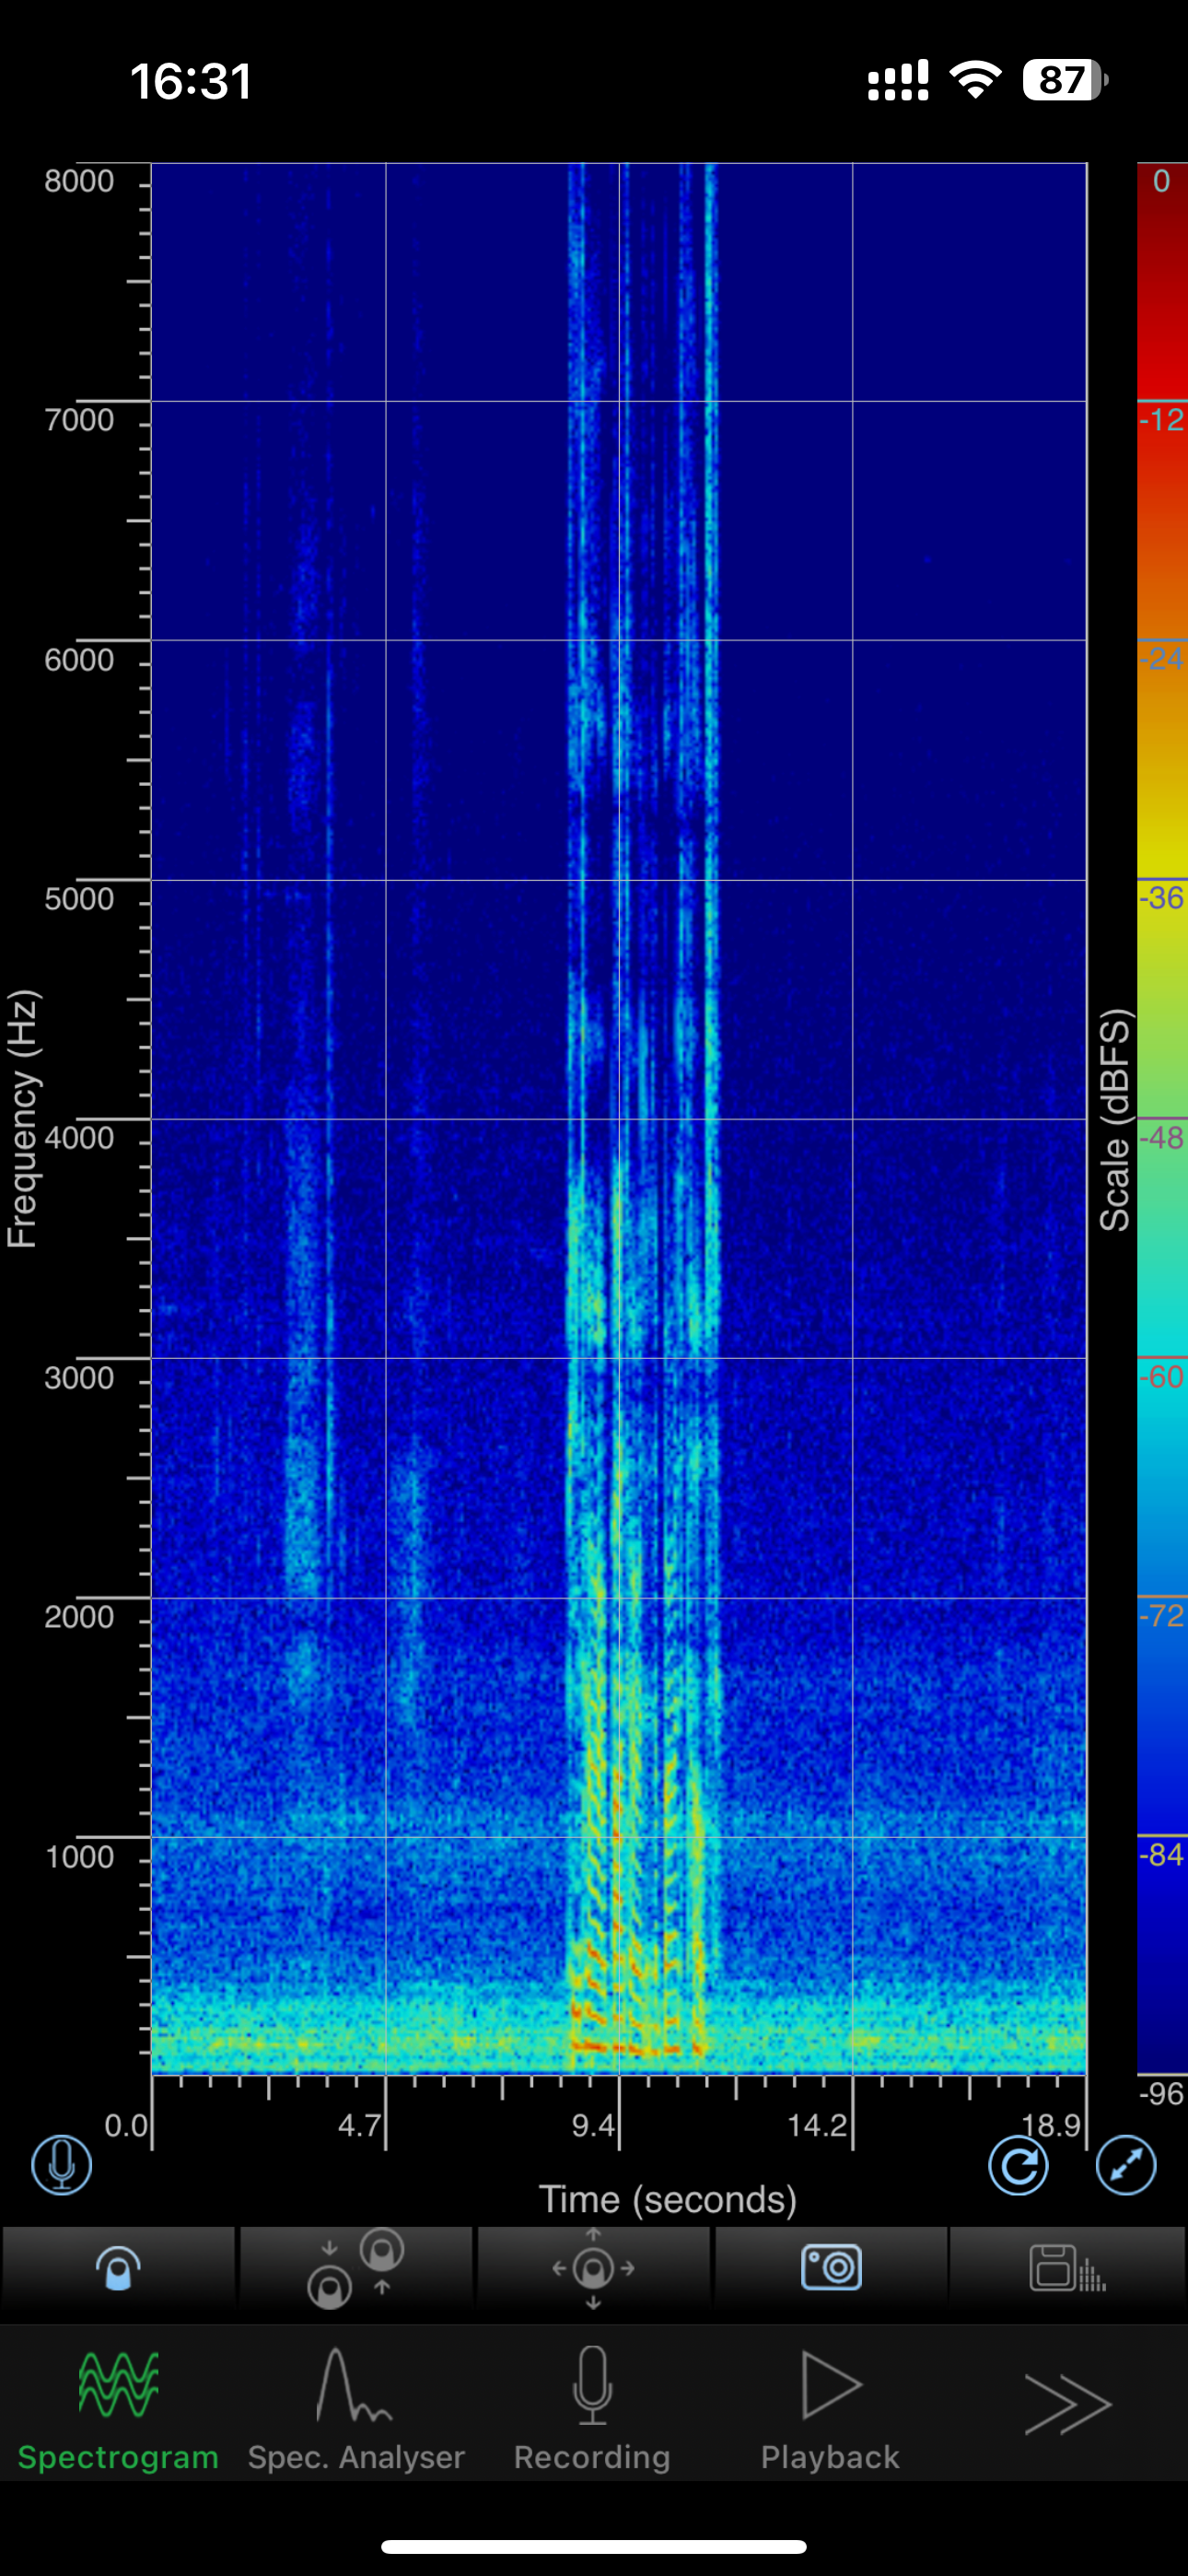
\includegraphics[width=0.4\textwidth]{./img/IMG_1831.PNG}
    \caption{Spectrogram of the sentence “Peter buttered the burnt toast”}
    \label{fig:Question1}
\end{figure}


Due to the inadequate scaling of the X-axis and Y-axis in the aforementioned figure, which does not effectively convey the desired experimental results, we have opted to utilize the recorded audio files and process them using relevant Python libraries.
The library used in this experiment is \texttt{librosa}. The code is shown in the following code block. The code reads the audio file, calculates the Short-Time Fourier Transform (STFT), and displays the spectrogram. The code also marks the voiced phonemes in the spectrogram.


\begin{figure}[H]
    \centering
    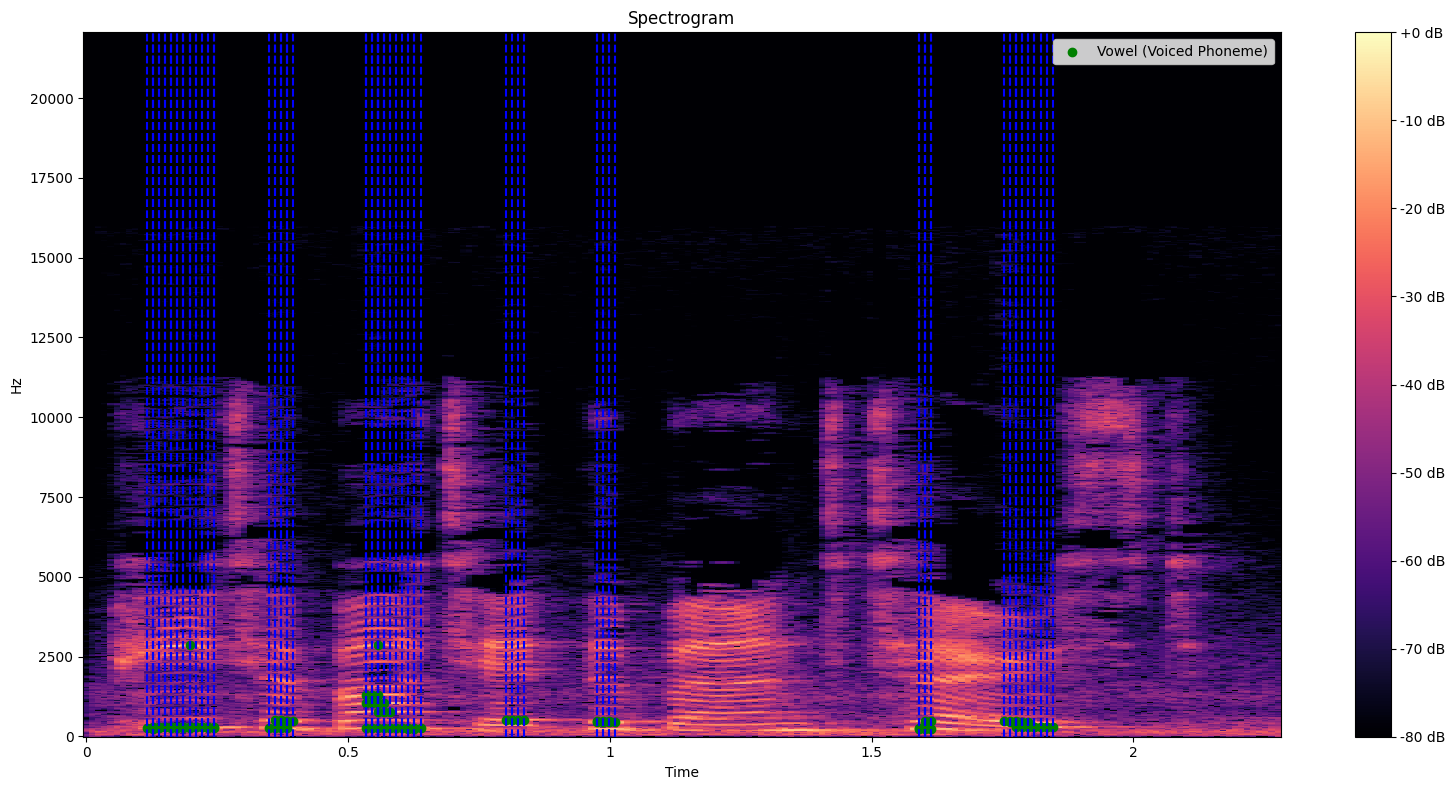
\includegraphics[width=\textwidth]{./img/Q1-1.png}
    \caption{Spectrogram of the sentence “Peter buttered the burnt toast”}
    \label{fig:Question1-2}
\end{figure}


From the figure \ref{fig:Question1-2}, the \textbf{green dots} and \textbf{blue line} indicate the sections corresponding to vowels (voiced phonemes). Additionally, there are several points where the frequency sharply rises; these points represent plosives, which are also known as stop consonants.

"Peter buttered the burnt toast" contains the following phonemes:

\begin{table}[H]
    \centering
    \begin{tabular}{|c|c|c|}
        \hline
        \textbf{Voiced Phonemes} & \textbf{Phonetic Representation} & \textbf{Count} \\ \hline
        Peter  & e, e & /i:/, /ə/ (2) \\ \hline
        buttered & u, ered & /ʌ/, /ɜ:/ (2) \\ \hline
        the & e & /ði:/ (1) \\ \hline
        burnt & u & /ɜ:/ (1) \\ \hline
        toast & oa & /əʊ/ (1) \\ \hline
        \textcolor{red}{\textbf{Total}} & & \textcolor{red}{7} \\ \hline
    \end{tabular}
    \caption{Phonemes in "Peter buttered the burnt toast"}
\end{table}

\vspace{1em} % Add some space between the tables
\begin{table}[H]
    \centering
    \begin{tabular}{|c|c|c|}
        \hline
        \textbf{Stop Consonants} & \textbf{Phonetic Representation} & \textbf{Count} \\ \hline
        Peter  & P, t & /p/, /t/ (2) \\ \hline
        buttered & b, t, d & /b/, /t/, /d/ (3) \\ \hline
        burnt & b, t & /b/, /t/ (2) \\ \hline
        toast & t, t & /t/, /t/ (2) \\ \hline
        \textcolor{red}{\textbf{Total}} & & \textcolor{red}{9} \\ \hline
    \end{tabular}
    \caption{Stop Consonants in "Peter buttered the burnt toast"}
\end{table}


/ð/ is a voiced dental fricative, representing the /th/ sound, as seen in the word "the." It does not belong to the categories of vowels or stop consonants; instead, it is classified as a fricative because the airflow creates friction between the tongue and the teeth during its production. In the spectrogram, there is a noticeable gap in the frequency domain.

Lastly, we can mark the voiced phonemes and stop consonants in the spectrogram. The updated spectrogram is shown in Figure \ref{fig:Question1-3}.

\begin{figure}[H]
    \centering
    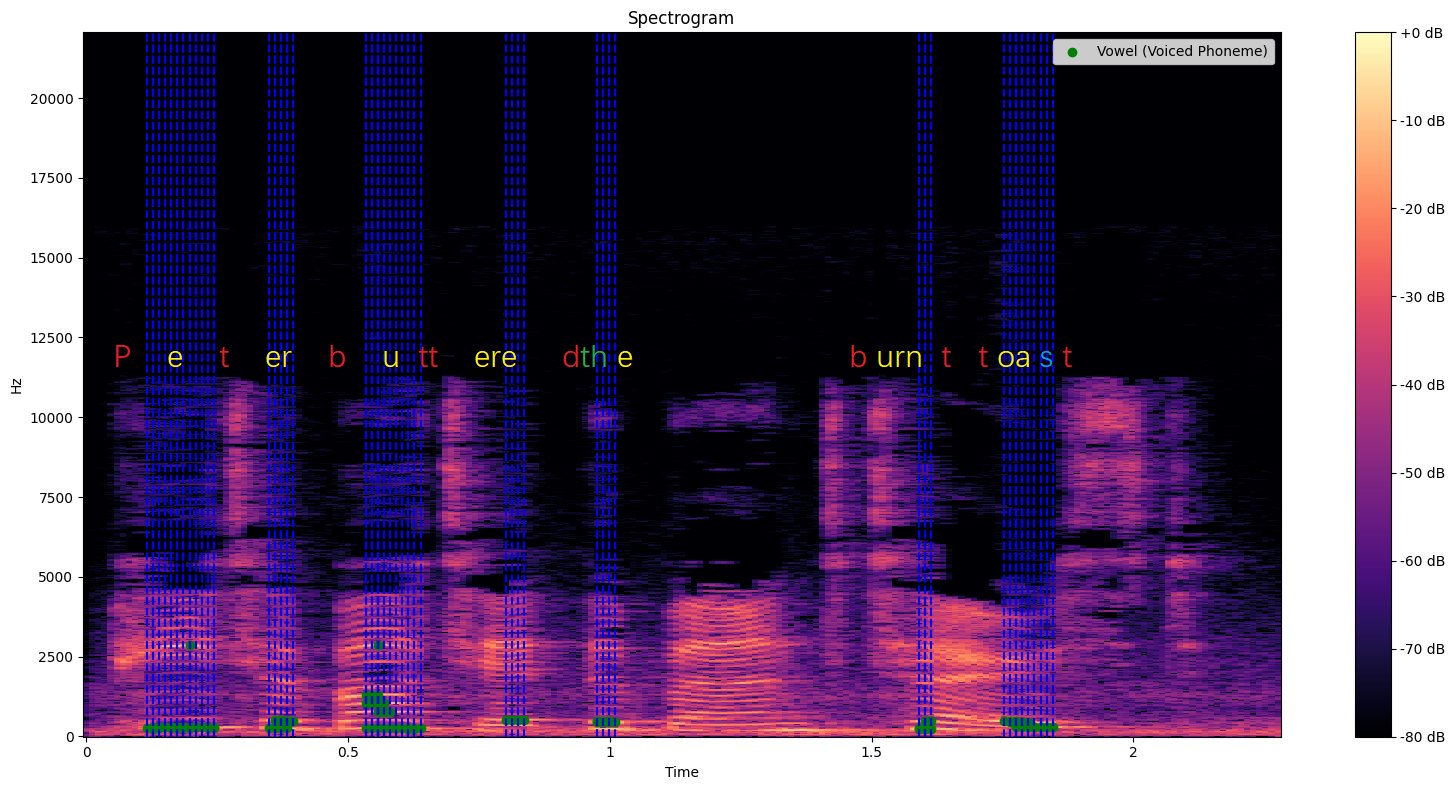
\includegraphics[width=\textwidth]{./img/Q1-2.png}
    \caption{Marked Spectrogram of the sentence “Peter buttered the burnt toast”}
    \label{fig:Question1-3}
\end{figure}

\subsection{Code}

\lstset{
    basicstyle=\small,
    breaklines=true,
    language=Python,
    showstringspaces=false,
    fontadjust=true
}
\begin{lstlisting}[language=Python, caption={Python code for Question 1}, label={code:Question1}, captionpos=b]
    import librosa
    import librosa.display
    import matplotlib.pyplot as plt
    import numpy as np

    # Read the audio file
    Q1, sr = librosa.load('./audio/Q1.wav', sr=44100)

    # Calculate the Short-Time Fourier Transform (STFT)
    D = librosa.amplitude_to_db(np.abs(librosa.stft(Q1)), ref=np.max)

    # Create a figure
    plt.figure(figsize=(16, 8))

    # Display the spectrogram
    librosa.display.specshow(D, sr=sr, x_axis='time', y_axis='linear')
    plt.colorbar(format='%+2.0f dB')
    plt.title('Spectrogram')

    # Define the frequency range for vowels
    vowel_freq_range = (200, 3000)
    threshold = -10

    # Get the frequencies
    freqs = librosa.fft_frequencies(sr=sr)
    vowel_indices = np.where((freqs >= vowel_freq_range[0]) & (freqs <= vowel_freq_range[1]))[0]

    # Find the high-energy indices
    high_energy_indices = np.where(D[vowel_indices, :] > threshold)

    # Convert the high-energy indices to time and frequency
    vowel_times = librosa.frames_to_time(high_energy_indices[1], sr=sr)
    vowel_freqs = freqs[vowel_indices[high_energy_indices[0]]]

    # Plot the voiced phonemes
    plt.scatter(vowel_times, vowel_freqs, color='g', marker='o', label='Vowel (Voiced Phoneme)')

    # Plot the stop consonants
    for time in vowel_times:
        plt.axvline(time, color='b', linestyle='--')

    # Add labels
    plt.legend(loc='upper right')

    # Display the plot
    plt.tight_layout()
    plt.show()
\end{lstlisting}

%
% End of Question 1

\newpage